\begin{figure}[htbp]
	\centering
	\resizebox{0.92\textwidth}{!}{%
		\begin{tikzpicture}[
			scale=1.0,
			>=latex,
			trave/.style={line width=1.2pt},
			diagM/.style={black, line width=0.8pt},
			diagMb/.style={gray!65, line width=1.0pt},
			hatch/.style={gray!40, line width=0.3pt},
			puntotang/.style={circle, fill=black, inner sep=1.2pt},
			richiamo/.style={gray!50!black, line width=0.3pt},
			]
			
			% ── Parametri geometrici (tratto generico [z_1, z_2]) ──
			\def\Ltratto{4}
			\pgfmathsetmacro{\xZ}{0}
			\pgfmathsetmacro{\xMid}{0.5*\Ltratto}
			\pgfmathsetmacro{\xZZ}{\Ltratto}
			
			% ── Scala verticale per ariosità ──
			\def\vscale{1.6}
			
			% Coordinate di disegno (conv. italiana: y_dis = -M)
			\pgfmathsetmacro{\yA}{0.5*\vscale}        % y_dis(z_1) = +0.5
			\pgfmathsetmacro{\yB}{-0.5*\vscale}       % y_dis(z_2) = -0.5
			\pgfmathsetmacro{\yMezz}{-0.4*\vscale}    % y_dis in mezzeria = -0.4
			\pgfmathsetmacro{\yRaccordo}{-0.8*\vscale}% y_dis vertice spezzata
			\pgfmathsetmacro{\yTangA}{0.1*\vscale}    % y_dis tangente parallela in z_1
			\pgfmathsetmacro{\yTangB}{-0.9*\vscale}   % y_dis tangente parallela in z_2
			\def\ylab{-1.95}
			
			% =========================================================
			% PANNELLO (a) — Tangenza agli estremi
			% =========================================================
			\begin{scope}[xshift=0cm]
				
				\draw[trave] (\xZ, 0) -- (\xZZ, 0);
				\node[below=2pt, font=\small] at (\xZ, 0) {$z_1$};
				\node[below=2pt, font=\small] at (\xZZ, 0) {$z_2$};
				\node[below=2pt, font=\small] at (\xMid, 0) {$z_G$};
				
				% Hatching della parabola
				\foreach \x in {0.10, 0.30, ..., 3.90} {
					\pgfmathsetmacro{\h}{(0.10*\x*\x - 0.65*\x + 0.5)*\vscale}
					\draw[hatch] (\x, 0) -- (\x, \h);
				}
				
				% Verticale di allineamento: baricentro z_G ↔ vertice della spezzata
				\draw[richiamo, dashed] (\xMid, 0) -- (\xMid, \yRaccordo);
				
				% Spezzata di sostituzione (caso b)
				\draw[diagMb]
				(\xZ, \yA) -- (\xMid, \yRaccordo) -- (\xZZ, \yB);
				
				% Parabola del momento (caso a)
				\draw[diagM]
				(\xZ, \yA)
				\foreach \x in {0.20, 0.40, ..., 3.80} {
					-- ({\x}, {(0.10*\x*\x - 0.65*\x + 0.5)*\vscale})
				}
				-- (\xZZ, \yB);
				
				% Punti di tangenza (cerchietti pieni agli estremi)
				\node[puntotang] at (\xZ, \yA) {};
				\node[puntotang] at (\xZZ, \yB) {};
				
				% Etichette dei valori del momento agli estremi
				\node[left=2pt, font=\small] at (\xZ, \yA) {$M(z_1)$};
				\node[right=2pt, font=\small] at (\xZZ, \yB) {$M(z_2)$};
				
				% Etichetta della parabola (sopra l'asse, agganciata alla curva)
				\draw[richiamo] (2.6, -0.82) -- (2.6, 0.45);
				\node[above, font=\footnotesize] at (2.6, 0.45) {parabola $M(z)$};
				
				% Etichetta della spezzata di sostituzione
				\draw[richiamo] (\xMid, \yRaccordo) -- (\xMid+0.9, \yRaccordo-0.35);
				\node[right, font=\footnotesize, gray!50!black]
				at (\xMid+0.9, \yRaccordo-0.35) {spezzata di sostituzione};
				
			\end{scope}
			
			% =========================================================
			% PANNELLO (b) — Tangenza in mezzeria
			% =========================================================
			\begin{scope}[xshift=7.5cm]
				
				\draw[trave] (\xZ, 0) -- (\xZZ, 0);
				\node[below=2pt, font=\small] at (\xZ, 0) {$z_1$};
				\node[below=2pt, font=\small] at (\xZZ, 0) {$z_2$};
				\node[below=2pt, font=\small] at (\xMid, 0) {$\tfrac{z_1+z_2}{2}$};
				
				\foreach \x in {0.10, 0.30, ..., 3.90} {
					\pgfmathsetmacro{\h}{(0.10*\x*\x - 0.65*\x + 0.5)*\vscale}
					\draw[hatch] (\x, 0) -- (\x, \h);
				}
				
				% Corda del diagramma
				\draw[diagMb, dashed] (\xZ, \yA) -- (\xZZ, \yB);
				% Tangente parallela alla corda in mezzeria
				\draw[diagMb, dashed] (\xZ, \yTangA) -- (\xZZ, \yTangB);
				
				% Parabola
				\draw[diagM]
				(\xZ, \yA)
				\foreach \x in {0.20, 0.40, ..., 3.80} {
					-- ({\x}, {(0.10*\x*\x - 0.65*\x + 0.5)*\vscale})
				}
				-- (\xZZ, \yB);
				
				\node[puntotang] at (\xZ, \yA) {};
				\node[puntotang] at (\xZZ, \yB) {};
				\node[puntotang] at (\xMid, \yMezz) {};
				
				\node[left=2pt, font=\small] at (\xZ, \yA) {$M(z_1)$};
				\node[right=2pt, font=\small] at (\xZZ, \yB) {$M(z_2)$};
				
				\draw[richiamo] (3.0, -0.45) -- (3.4, 0.20);
				\node[above, font=\footnotesize, gray!50!black] at (3.4, 0.20) {corda};
				
				\draw[richiamo] (3.0, -1.04) -- (3.4, -1.60);
				\node[below, font=\footnotesize, gray!50!black] at (3.4, -1.60)
				{tangente parallela};
				
				\draw[richiamo] (\xMid-0.05, \yMezz-0.05) -- (\xMid-0.9, \yMezz-0.4);
				\node[left, font=\footnotesize] at (\xMid-0.9, \yMezz-0.4)
				{punto di tangenza};
				
			\end{scope}
			
		\end{tikzpicture}
	}
	\caption{Le due proprietà di tangenza del diagramma del momento su un
		tratto generico $[z_1, z_2]$ di una trave sotto carico uniforme.
		(a)~\emph{Tangenza agli estremi:} la parabola del momento (linea
		nera) e la spezzata di sostituzione (linea grigia continua),
		ottenuta sostituendo il carico distribuito con la sua risultante
		applicata nel baricentro $z_G$ del tratto, sono tangenti agli
		estremi $z_1$ e $z_2$, dove i valori del momento e le pendenze
		coincidono; la spezzata si raccorda sulla verticale di $z_G$.
		(b)~\emph{Tangenza in mezzeria:} la corda che congiunge le ordinate
		del diagramma in $z_1$ e $z_2$ (tratto grigio tratteggiato
		superiore) è parallela alla tangente alla parabola in mezzeria
		$(z_1+z_2)/2$ (tratto grigio tratteggiato inferiore).}
	\label{fig:stat_tangenze}
\end{figure}
